\documentclass[report.tex]{subfiles}
\begin{document}
\subsection{Theoretical background}

Impedance matching can be achieved through analytical methods, but graphical methods prove to be most efficient; especially  with the help of Smith charts.

An RF network ($f=1~GHz$) with a complex input impedance of $Z_{in}=(455-j227)~\Omega$, in a system with the characteristic impedance $Z_0=50 ~\Omega$ has the have a matching input network. To determine this matching network, the source load ($Z_0$) and the complex conjugate of the input impedance ($Z_{in}^*$) is normalized with respect to $Z_0$.
\begin{equation*}
%\label{eqn:z_in}
z_0=Z_0/Z_0 = 1~\Omega
\end{equation*}
\begin{equation*}
z_{in}^*=Z_{in}^*/Z_0=(9.1-4.54)~\Omega
\end{equation*}

Then, by following the resistance and conductance lines of the Smith chart \emph{from} the normalized source load \emph{to} $z_{in}^*$, as shown in fig.~\ref{fig:input_matching_smith_chart}, the reactance of the matching network is determined by point A.

\begin{figure}[h]
    \centering
    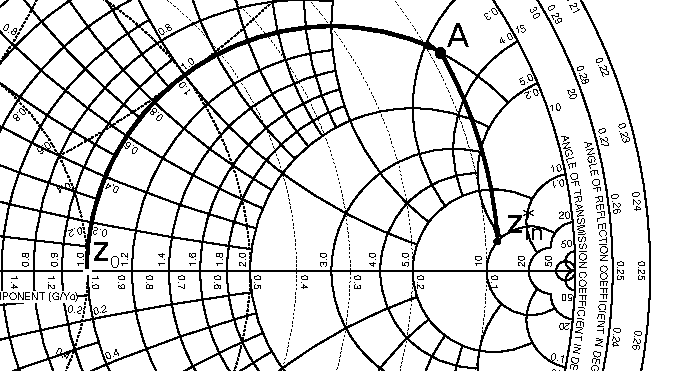
\includegraphics[scale=0.9]{input_matching_ZY_chart_ver2}
    \caption{Input matching in Smith chart}
    \label{fig:input_matching_smith_chart}
\end{figure}

Depending on the path chosen from $z_0$ to $z_{in}^*$, different matching networks are generated, as shown in table \ref{tab:relations}. In the case of fig.~\ref{fig:input_matching_smith_chart}, the matching network would consist of a series inductor and a shunt capacitor.

\begin{table}[h]
\centering
\caption{Smith chart line and rotation correlation matrix}
\label{tab:relations}
\begin{tabular}{l | l l}
                & Clockwise & Counterclockwise \\
\hline
Resistance line & Series inductor   & Series capacitor\\
Conductance     & Shunt Capacitor & Shunt inductor \\
\end{tabular}
\end{table}

At point A in fig.~\ref{fig:input_matching_smith_chart}, $X_C=1/0.225=4.44~\Omega$ and $X_L=3.3~\Omega$. From these reactances, $C$ and $L$ can be calculated and de-normalized:
\begin{equation*}
X_C Z_0 = \frac{1}{\omega \tilde{C}} \implies \tilde{C} = \frac{1}{\omega X_C Z_0} \approx 0.716 ~pF
\end{equation*}
\begin{equation*}
X_L Z_0=\omega \tilde{L} \implies \tilde{L}=\frac{X_L Z_0}{\omega} \approx 26.3~nH
\end{equation*}

Figure~\ref{fig:input_matching_network} show the resulting input matching network connected to a testbench ($701~fF$ corresponds to $-227~\Omega$). The S-parameter simulation in fig.~\ref{fig:fig:S-params_matching_network} show that for $f=1GHz$, the reflection coefficient is close to 0.

\begin{figure}
    \centering
    \subfloat[] {
        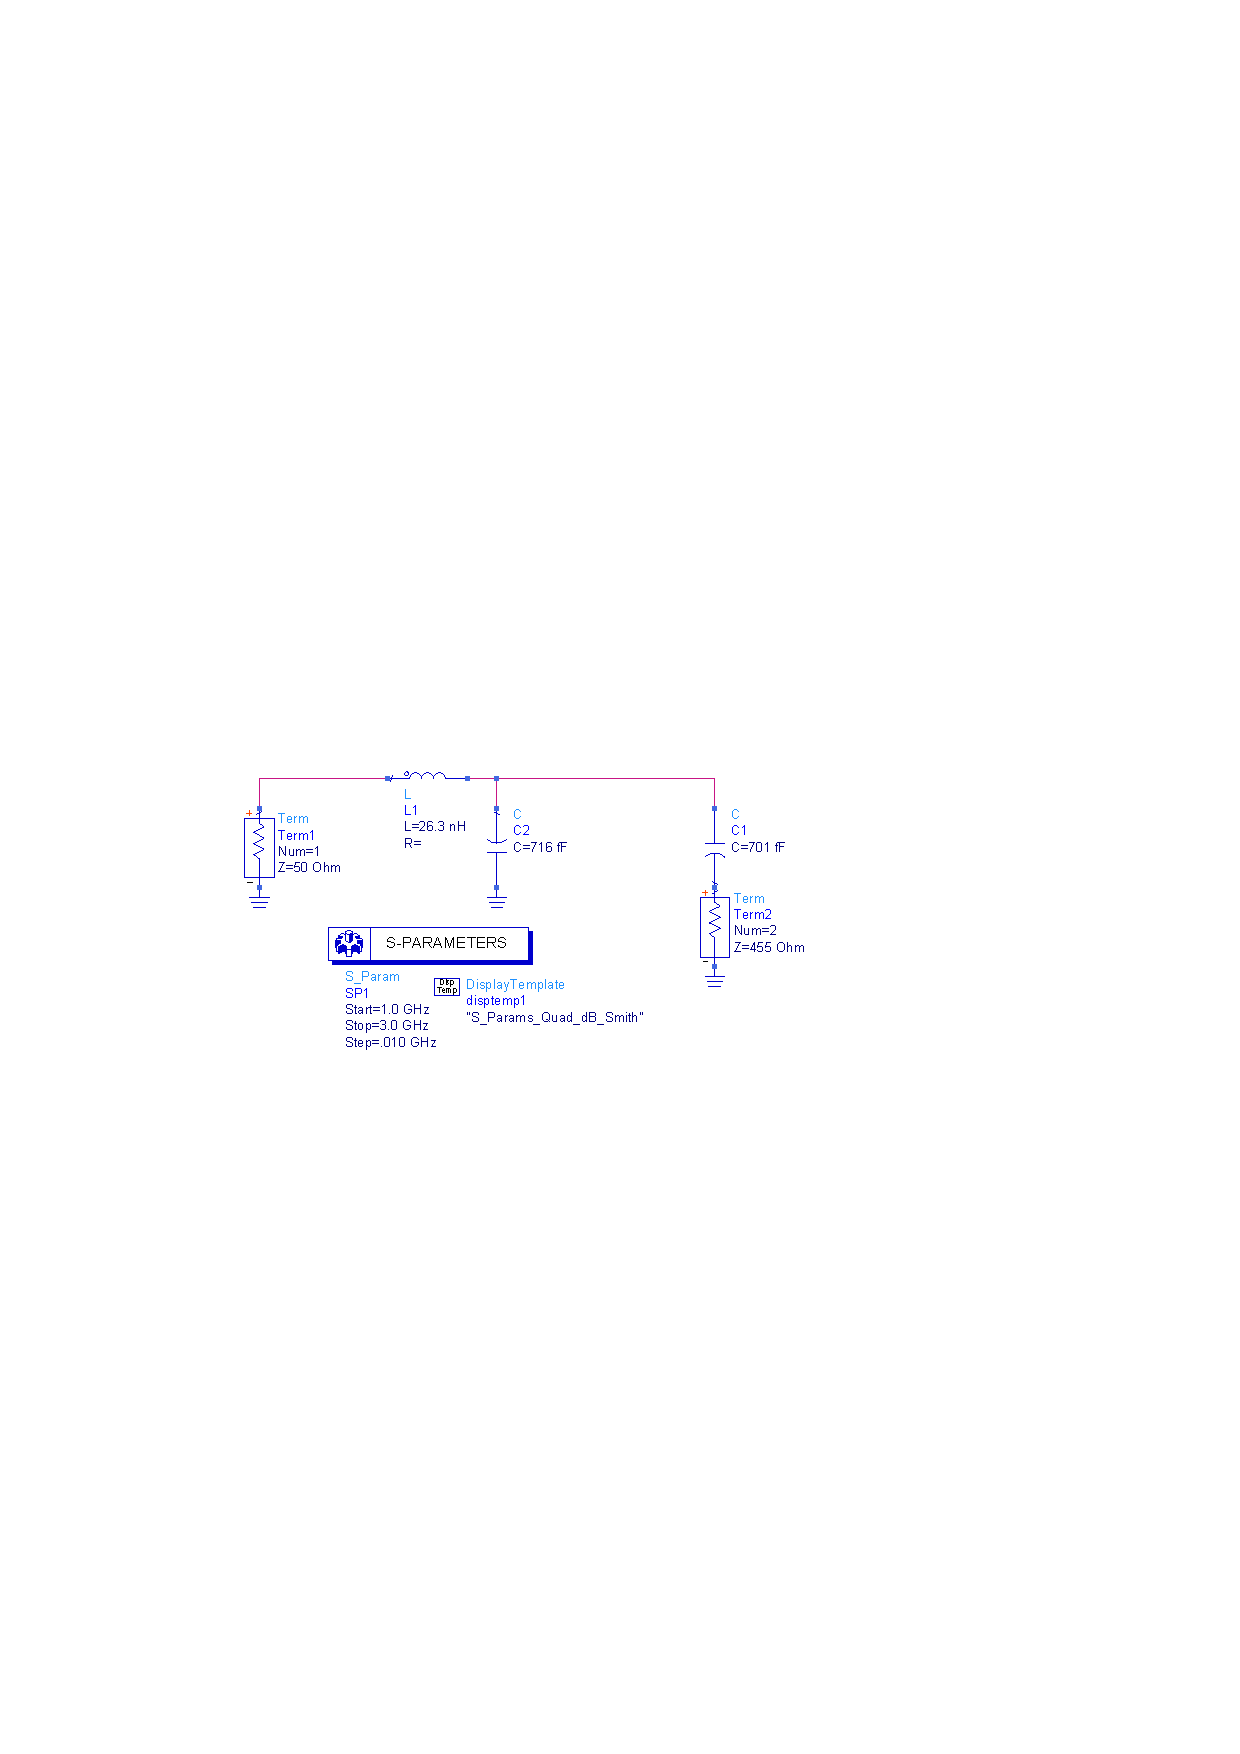
\includegraphics{prep_work_simulation_circuit}
        \label{fig:input_matching_network}
    }
    
    \subfloat[] {
        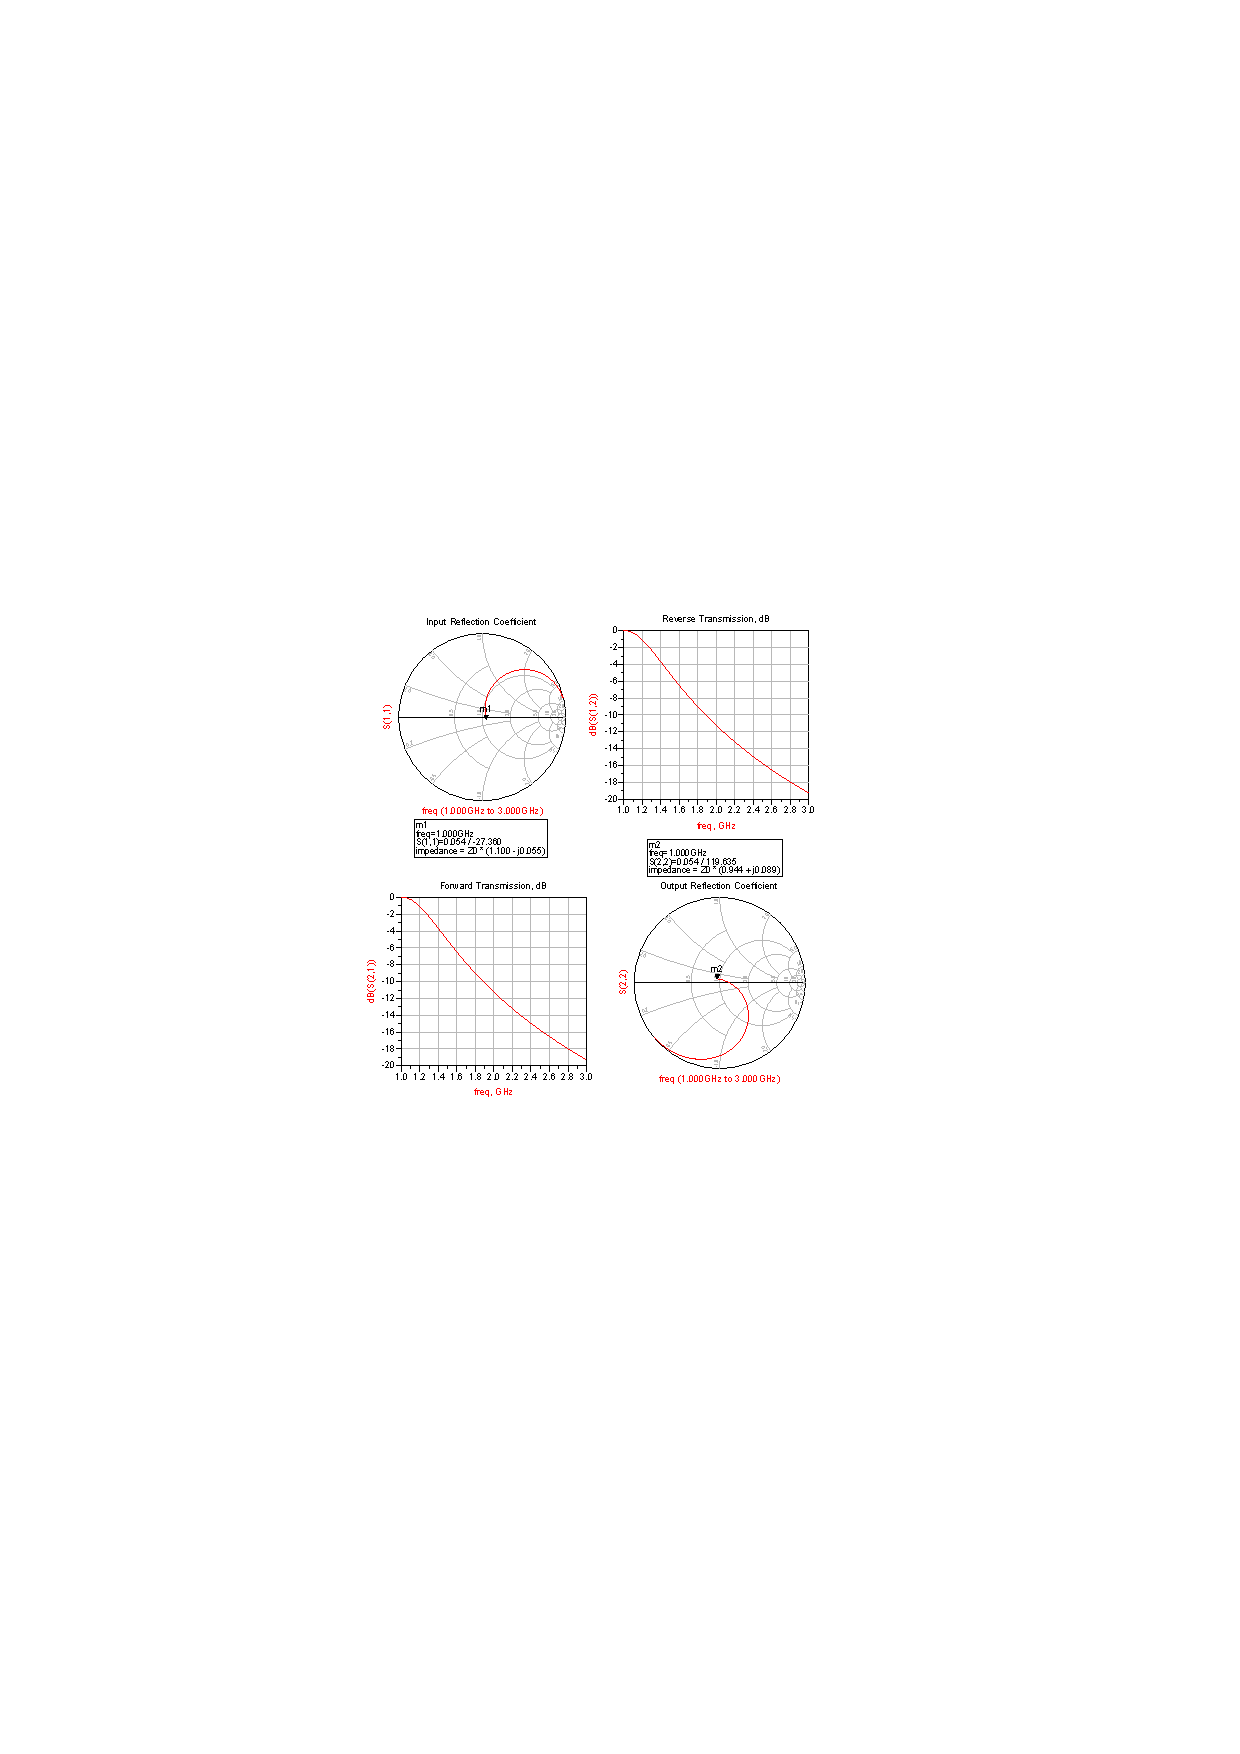
\includegraphics[scale=1.4]{S-params_prep_work}
        \label{fig:fig:S-params_matching_network}
    }
    \caption{Simulation setup and result of an input matching network}
\end{figure}

\clearpage % DO NOT REMOVE! The above figure becomes displaced otherwise

\end{document}
